%% ID: A1989PIQ5a
%% TITLE: Pulling Out a Nail
%% TYPE: question
%% QUESTIONTYPE:  scq
%% CONCEPTS: forces, vectors2
%% VIDEOS: 
%% LEVEL: 2
%% TOPIC: mechanics/statics
%% ORDER: 3

\begin{problem}[A1989PIQ5a]
%Diagram removed
{\exposition{A nail is embedded into a wooden post. A cord is used to pull the nail out; it is attached to the head of the nail and pulls at an angle of 30$^{\circ}$ to the post with a tension of 50 N.} \question{What is the force tending to pull the nail out of the post?}
\begin{enumerate}
	\item \choice[a]{$50\cos{30^{\circ}}$}
	\item  \choice[b]{$50\sin{30^{\circ}}$}\correct
	\item  \choice[c]{$50\tan{30^{\circ}}$}
	\item  \choice[d]{$50/\cos{30^{\circ}}$}
	\item  \choice[e]{$50/\sin{30^{\circ}}$}
\end{enumerate}
}
{\textit{Used with permission from UCLES, A Level Physics, June 1989, Paper 1, Question 5.}}
{\answer{The correct answer is (b).} As is Figure \ref{fig:Statics_force_nail}, to take the horizontal component of the tension, multiply by $\sin{30^{\circ}}$.

\begin{figure}[h]
	\centering
	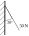
\includegraphics[width=0.15\textwidth]{Statics_force_nail}
	\caption{}
	\label{fig:Statics_force_nail}
\end{figure}
}
\end{problem}